\documentclass[11pt]{article}
\usepackage[utf8]{inputenc}
\usepackage[T1]{fontenc}
\usepackage{amsmath,amssymb,amsthm}
\usepackage{booktabs}
\usepackage{graphicx}
\usepackage[margin=2.7cm]{geometry}
\usepackage{hyperref}
\usepackage{tikz}
\usetikzlibrary{positioning,arrows.meta,calc}
\tikzset{
  ax/.style={draw=blue!60!black, fill=blue!12, rounded corners=2pt, font=\scriptsize, inner sep=3pt, minimum height=5.5mm},
  th/.style={draw=blue!60!black, fill=blue!6, rounded corners=2pt, font=\scriptsize, inner sep=3pt, minimum height=5.5mm},
  goal/.style={draw=green!50!black, fill=green!14, rounded corners=3pt, font=\scriptsize\bfseries, inner sep=3.5pt},
  open/.style={draw, dashed, rounded corners=2pt, font=\scriptsize, inner sep=3pt},
  fl/.style={-{Stealth[length=2mm]}, gray!70},
  gl/.style={-{Stealth[length=2.2mm]}, green!50!black, thick},
}

% ============================================================================
% REGLE D'OR (PLAN.md) : chaque phrase adossee a un objet du depot.
% Les commentaires %% ANCRE: pointent la preuve de chaque section.
% Article A3 du plan editorial docs/articles/PLAN_ARTICLES.md.
% ============================================================================

\newtheorem{definition}{Definition}
\newtheorem{proposition}{Proposition}
\theoremstyle{remark}\newtheorem{remark}{Remark}

\title{Charting the Open:\\
Certified Reductions of Goldbach's Conjecture,\\
and a Measurement of What They Do Not Contain}

\author{Karl [full name]\thanks{ISEP Paris. Contact: [email]. Code and certified
corpus: [repository URL and tagged commit hash at submission time]. All measurements
in this paper were re-run in a fresh process on 19 August 2026; the replay script is
\texttt{recherche/goldbach/capstone.py}.}}

\date{Preprint --- August 2026}

\begin{document}
\maketitle

\begin{abstract}
What can a kernel-verified system produce on a problem it cannot solve? We report a
four-month campaign in which Goldbach's conjecture was written over the constructed
cardinal arithmetic of an LCF kernel built on Bourbaki's own formalism, and then
reduced --- never proved. The campaign yields a \emph{certified map}: eighteen
kernel-judged links, replayable in a fresh process, collapsing three independent lines
of attack onto a single object, so that proving the conjecture reduces to proving that
for every composite $k$ the primes below $2k$ meet their additive mirror. Two
structural facts are certified about that meeting: its solutions come in pairs under
the involution $m \mapsto 2k-m$, and one member of each pair lies in the lower half,
so searching half the interval suffices. Our central result is negative and
\emph{measured}: re-deriving those reductions with the primality predicate replaced by
a \emph{parameter}, the same proofs close verbatim on a totally opaque set, on
primality, and on a predicate for which the question is trivial. Reductions that
cannot distinguish the primes from a structureless set cannot prove Goldbach --- and
this is a property of the statements, not a defect of the proofs. The measurement
explains, at one stroke, two further paths we had already closed negatively: raw
counting and equational reasoning both fail because neither ever looks at \emph{which}
integers are prime. We also report a certified fidelity defect --- the repository's
primality predicate did not constrain its argument to be an integer, making the
formalized conjecture strictly weaker than the conjecture --- proved in the kernel and
repaired at provably zero cost on numerals. We claim no arithmetic progress: the
conjecture is exactly as open as before. We claim that a verified system can
\emph{delimit} an open problem --- draw in code, rather than by estimation, the line
where the structural ends and the arithmetic begins --- and that this is a mathematical
object rather than a report of failure.
\end{abstract}

%% ============================================================================
\section{Introduction}
%% ANCRE: PLAN.md (article/goldbach/) table des revendications G1-G9 ;
%% docs/articles/CARTE_GOLDBACH.md ; recherche/README.md
%% ============================================================================

A proof assistant is an instrument for closing goals. Pointed at an open problem it
does the only thing it can: it fails, repeatedly, and the record of that failure is
conventionally discarded. The question this paper asks is what such an instrument can
be made to \emph{produce} when success is excluded in advance --- not as consolation,
but as a mathematical result.

Our answer has three parts, and the third is the one we consider new. First, a
verified system can produce a \emph{map}: a network of certified equivalences and
reductions, each link a kernel object, with the remaining obligation stated exactly at
every leaf. Second, it can close paths \emph{negatively}, and record why. Third --- and
this is what the map alone cannot do --- it can \emph{measure how much of the problem
its own reductions actually touch}. We do this by parameterizing: the predicate
``is prime'' is replaced by an opaque parameter $S$, and the reductions are re-derived.
Those that still close have been shown, by execution rather than by argument, to
contain no arithmetic at all.

That measurement changes the epistemic status of a body of reduction work. A
reduction that closes for every $S$ is not a step toward Goldbach and never could have
been; it is a statement about additive structure that the primes merely instantiate.
Knowing which of one's results are of this kind --- and knowing it mechanically, at the
cost of a few seconds per instance --- is the difference between a research program that
is exploring and one that is circling.

\paragraph{The setting sharpens the experiment.} We work in an LCF-style kernel
implemented over Bourbaki's own formal system: the $\tau$ operator, its abbreviated
assemblies, and the body of criteria Bourbaki \emph{proves} about proofs rather than
posits as rules. The arithmetic is the corpus's own constructed cardinal arithmetic,
not a primitive type of naturals. Two consequences matter here. The oracle is
\emph{exact}: every claim below is a kernel object or a stated measurement, never an
estimate. And because $\exists x\,\varphi(x)$ \emph{is} $\varphi(\tau x\,\varphi)$ in
Bourbaki's system rather than a separate quantifier, the conjecture can be rewritten
with no existential quantifier at all --- three properties of two named terms
(Section~\ref{sec:map}). That is not available in a conventional setting, and it turns
out to be the form in which the machine's own search organs later re-derive the
statement unaided.

We report the campaign honestly, which means reporting that it did not work. Goldbach
is open. Every theorem below is of the form $X \Rightarrow \mathrm{Goldbach}$ or
$\mathrm{Goldbach} \Leftrightarrow Y$, and a test in the repository fails if any
exported result ever concludes the conjecture alone (Section~\ref{sec:repro}).

\paragraph{Contributions.}
\begin{enumerate}\itemsep2pt
\item \textbf{A certified map of an open problem} (Section~\ref{sec:map}): eighteen
kernel-judged links, replayed in a fresh process in about seven and a half minutes,
under which three independent lines of attack --- a bounded verification for
$n \le 86$, a reduction to composite $k$, and a sieve reformulation --- collapse onto a
single object. Proving the conjecture reduces to proving that for every composite $k$,
the primes $\le 2k$ meet their additive mirror.
\item \textbf{Goldbach without $\exists$} (Section~\ref{sec:map}): using Bourbaki's
$\tau$, the conjecture becomes three properties of two named terms. Both directions are
certified.
\item \textbf{A measurement of arithmetic content} (Section~\ref{sec:abstract}, our
central result): with the primality predicate as a parameter, the symmetry and
half-interval reductions close verbatim on an opaque predicate, on primality, and on a
trivial predicate. ``Goldbach is an instance'' is an execution, not a claim of prose.
\item \textbf{Two paths closed negatively, with a common cause}
(Section~\ref{sec:negative}): raw counting and equational strengthening both fail, and
the parameterization of the previous item explains why --- neither ever inspects which
integers are in $S$.
\item \textbf{A certified fidelity defect and its repair} (Section~\ref{sec:fidelity}):
the repository's primality predicate guarded only the divisor, so the formalized
conjecture quantified over non-integer witnesses and was strictly weaker than the
conjecture. The defect is a kernel theorem; the repair is proved free on numerals.
\item \textbf{Two guards against the only cheating available here}
(Section~\ref{sec:repro}): a column separating ``closed'' from ``axiom-free'' --- eleven
of eighteen links are free, seven rest on the sieve's two dedicated axioms --- and a
test that fails if anything in the research folder concludes the conjecture.
\end{enumerate}

\paragraph{What we do not claim.} No new arithmetic fact about the primes is
established. The negative results of Section~\ref{sec:negative} are measurements, not
impossibility theorems: the counting result is a numerical observation about $\pi$, and
the equational result is an observation about the shape of a gap produced by
\emph{our} organs at a given state. Section~\ref{sec:abstract} does not show Goldbach
unprovable by these methods in any logical sense; it shows that proofs which do not
distinguish $S$ from a structureless set cannot establish a statement that does depend
on $S$. That is a delimitation, not a lower bound.

%% ============================================================================
\section{Background: the kernel, and an arithmetic that must be guarded}
\label{sec:background}
%% ANCRE: bourbaki/i_* ; recherche/README.md ; article/main.tex sec:background
%% ============================================================================

We summarize only what this paper needs; the kernel, its trust boundary, and the
instrumentation around it are the subject of a companion paper.

The kernel is LCF-style: a value of type \texttt{Theoreme} is constructible only
through kernel primitives, and the repository forbids fabricating one by any other
route. A theorem is \emph{closed} when its hypothesis set is empty. Theories are
Bourbaki's: a named finite set of explicit axioms. The reference theory of sets carries
22 axioms, and that count is asserted at every execution of every script in this paper.

Two features of the substrate shape everything below.

\paragraph{Arithmetic is constructed, and cardinal.} There is no primitive type of
natural numbers. Integers are finite cardinals, and the additive laws available are
those of cardinal arithmetic. This is not a stylistic choice --- it is the book's
development --- and it has a sharp consequence for statement fidelity: a quantifier
that the author believes ranges over integers in fact ranges over cardinals unless a
finiteness guard is written. Section~\ref{sec:fidelity} reports what that cost, and
Section~\ref{sec:structure} reports a case where omitting the guard would have made a
statement \emph{false} rather than merely unprovable, since additive cancellation fails
for infinite cardinals: $\aleph_0 + 1 = \aleph_0 + 2$ while $1 \neq 2$.

\paragraph{The existential quantifier is not primitive.} In Bourbaki's system,
$(\exists x)\varphi(x)$ is an abbreviation for $\varphi(\tau x\,\varphi)$. The kernel
exposes this directly, so an existential goal can be traded for properties of an
explicitly named term. Section~\ref{sec:map} uses this to rewrite the conjecture
without any existential quantifier; the same mechanism is what lets a search organ
later perform that rewriting on its own.

\paragraph{Where the results live.} The repository's main tree mirrors the book's table
of contents, so that an empty directory is a coverage hole. Goldbach is not in
\emph{Theory of Sets}. Results proved beyond the book therefore live in a separate
\texttt{recherche/} tree, exempt from the book-anchoring discipline but subject to
\emph{identical} kernel rules: same primitives, no fabricated theorems, 22 axioms
asserted throughout. A research result is not less certified --- it is only off-book.

%% ============================================================================
\section{The certified map}
\label{sec:map}
%% ANCRE: recherche/goldbach/{enonces,crible,pont_tau,composes,synthese}.py ;
%% capstone.py::verifie_chaine (18/18 CLOS, mesure du 19 aout) ;
%% docs/articles/CARTE_GOLDBACH.md sections 1-5
%% ============================================================================

Write $H$ for the ``halves'' form of the conjecture --- for every finite $k \notin
\{0,1\}$, $k+k$ is a sum of two primes --- which the campaign proved interderivable
with the repository's statement. The map's business is to move $H$ to a form where
what is missing is isolated at one point.

\subsection{Four equivalent forms}

\begin{center}
\begin{tabular}{@{}llll@{}}
\toprule
form & statement & status & module \\
\midrule
DEP & the repository's \texttt{goldbach()} & reference & \texttt{enonces.py} \\
$H$ & halves: $(\forall k)\,\mathrm{decomp}(k{+}k)$ & $\Leftrightarrow$ DEP & \texttt{enonces.py} \\
HC & halves, restricted to composite $k$ & $\Leftrightarrow H$ (GG7) & \texttt{composes.py} \\
$H_\tau$ & canonical: no $\exists$ at all & $\Leftrightarrow H$ (GG9/GG10) & \texttt{pont\_tau.py} \\
\bottomrule
\end{tabular}
\end{center}

\paragraph{Composites are the whole problem.} If $k$ is prime then $2k = k+k$ decomposes
for free, so the conjecture bears only on composite $k$. The proof is excluded middle on
$\mathrm{prime}(k)$, with the prime branch discharged through the family $\{2p\}$ and an
$\alpha$-renaming bridge --- the repository's statement forces two distinct spellings of
\texttt{est\_premier}, and the bridge crosses between them. That bridge will reappear in
Section~\ref{sec:abstract} as an artifact rather than a step.

\paragraph{The conjecture without an existential quantifier.} Applying
$(\exists x)\varphi \equiv \varphi(\tau x\,\varphi)$ twice, with
$T := \tau p\,(\exists q\;\mathrm{mat})$ and $Q := \tau q\,(\mathrm{mat}[p := T])$, the
conjecture becomes
\[
\mathrm{prime}_1(T) \;\wedge\; \mathrm{prime}_2(Q) \;\wedge\; 2k = T + Q ,
\]
three properties of two named terms. Both directions are certified and free of ad-hoc
axioms. Nothing is gained mathematically --- no information is created --- but the
\emph{shape} of the question changes, from ``does a witness exist'' to ``does a named
term have these properties''. We note in passing, since it belongs to the companion
paper, that the campaign's search organs later reconstructed exactly this move on their
own: a witness-\emph{proposing} organ that fabricates $\tau x(\varphi)$ from the goal
alone turns the reported gap on a decomposition goal from the intact existential
statement into a statement about the properties of a named term.

\subsection{The sieve, and the convergence}

Let
\[
P_{2k} := \{\, p : \mathrm{prime}(p) \wedge p \in [0,2k] \,\},
\qquad
Q_{b} := \{\, x : (\exists y)(\mathrm{prime}(y) \wedge b = x + y) \,\}
\]
--- the primes below $2k$, and the \emph{additive mirror} of $b$. Both are opaque terms
characterized by axioms of a dedicated theory (Section~\ref{sec:repro} accounts for
them). The mirror is defined by an internal existential: no subtraction, no
commutativity, no cardinality of a complement is used.

\begin{proposition}[sieve equivalence, GG19, both directions]
$\vdash (\forall k)\bigl[\, (\exists m)(m \in P_{2k} \wedge m \in Q_{2k})
\;\Longleftrightarrow\; 2k = p+q \text{ with } p,q \text{ prime} \,\bigr]$.
\end{proposition}

Write $\mathrm{meet}(k)$ for the left-hand side. The forward direction is derivable only
with the \emph{guarded} statement of Section~\ref{sec:fidelity}: it consumes finiteness
of $p$. This is worth recording, because it is the pattern by which a fidelity defect
announces itself --- the guard is not decorative, the proof demands it.

The map's payoff is that everything the campaign proved lands on $\mathrm{meet}$:

\begin{center}
\begin{tabular}{@{}lll@{}}
\toprule
line of attack & what it had & absorbed by \\
\midrule
bounded & Goldbach verified for all $n \le 86$ & GG25 --- a concrete witness gives the meeting \\
composites & prime $k$ are free & GG22 --- $m := k$ witnesses \\
sieve & $P_{2k}$ meets its mirror & the arrival form \\
\bottomrule
\end{tabular}
\end{center}

\begin{proposition}[synthesis, GG24]
$\vdash \bigl[\,(\forall k)\;(\text{$k$ finite, composite}) \Rightarrow \mathrm{meet}(k)\,\bigr]
\;\Longrightarrow\; H .$
\end{proposition}

Three scattered formulations became one goal. We state the obvious reservation in the
repository's own words: this is an implication whose hypothesis is not proved, and that
hypothesis \emph{is} the conjecture restricted to composites. The value is in
designating a single object to attack, not in having attacked it.

\begin{figure}[t]
\centering
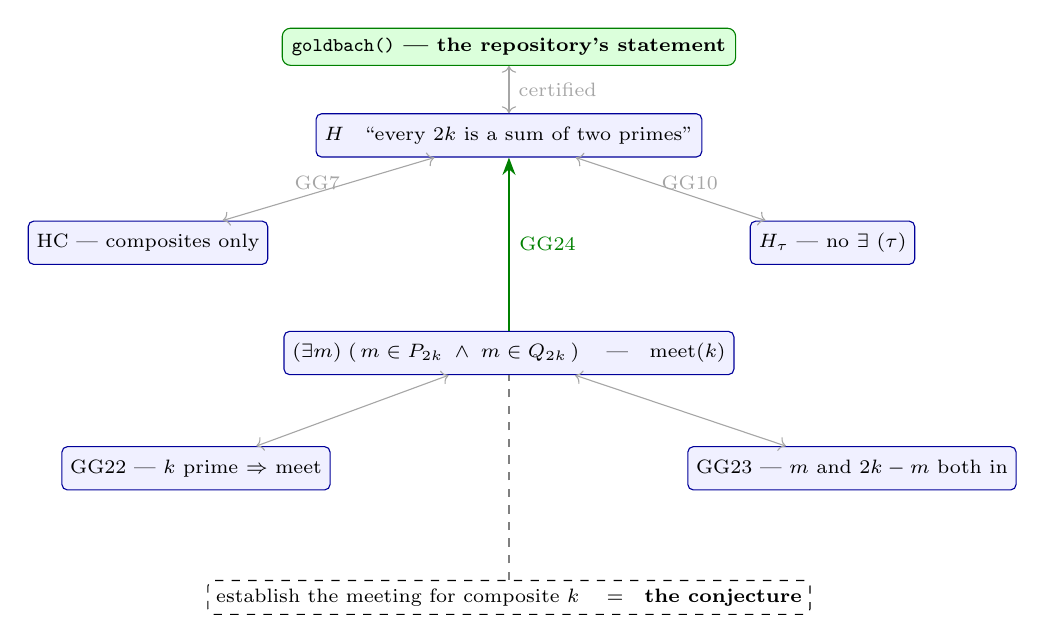
\begin{tikzpicture}[node distance=6mm and 10mm]
\node[goal] (dep) {\texttt{goldbach()} --- the repository's statement};
\node[th, below=of dep] (h) {$H$ \;\;``every $2k$ is a sum of two primes''};
\node[th, below left=8mm and 6mm of h] (hc) {HC --- composites only};
\node[th, below right=8mm and 6mm of h] (ht) {$H_\tau$ --- no $\exists$ ($\tau$)};
\node[th, below=22mm of h] (meet) {$(\exists m)\;(\,m \in P_{2k} \;\wedge\; m \in Q_{2k}\,)$ \;\; --- \; $\mathrm{meet}(k)$};
\node[th, below left=9mm and -6mm of meet] (gg22) {GG22 --- $k$ prime $\Rightarrow$ meet};
\node[th, below right=9mm and -6mm of meet] (gg23) {GG23 --- $m$ and $2k-m$ both in};
\node[open, below=26mm of meet] (openn) {establish the meeting for composite $k$ \;\; = \; \textbf{the conjecture}};
\draw[fl,<->] (dep) -- node[right,font=\scriptsize] {certified} (h);
\draw[fl,<->] (h) -- node[left,font=\scriptsize,pos=.4] {GG7} (hc);
\draw[fl,<->] (h) -- node[right,font=\scriptsize,pos=.4] {GG10} (ht);
\draw[gl] (meet) -- node[right,font=\scriptsize] {GG24} (h);
\draw[fl,<->] (meet) -- (gg22);
\draw[fl,<->] (meet) -- (gg23);
\draw[dashed,gray] (openn) -- (meet);
\end{tikzpicture}
\caption{The map. Solid arrows are kernel-certified; the dashed link is the conjecture.
$P_{2k}$ is non-empty and finite (proved); $Q_{2k}$ is its additive mirror. Every
certified link is replayed by \texttt{capstone.py} and judged by the kernel.}
\label{fig:map}
\end{figure}

%% ============================================================================
\section{The structure of the meeting}
\label{sec:structure}
%% ANCRE: recherche/goldbach/symetrie.py (GG23) ; demi.py (demi_intervalle,
%% rencontre_se_restreint) ; CARTE_GOLDBACH.md sections 10-11
%% ============================================================================

Two facts are certified about $\mathrm{meet}$. Neither says anything about existence;
both constrain the shape of the solution set.

\begin{proposition}[symmetry, GG23]
$\vdash (\forall k)(\forall m)\bigl[\, m \in P_{2k} \cap Q_{2k} \Rightarrow
(\exists m')\bigl(m' \in P_{2k} \cap Q_{2k} \wedge 2k = m + m'\bigr) \,\bigr].$
\end{proposition}

Solutions come in pairs, stable under the involution $m \mapsto 2k - m$ whose fixed
point is $k$ --- exactly the case GG22 handles. Goldbach decompositions go two by two.

\begin{proposition}[the half suffices]
$\vdash (\forall k)\bigl[\,k \text{ finite} \Rightarrow
\bigl(\mathrm{meet}(k) \Leftrightarrow (\exists m)(m \in P_{2k} \cap Q_{2k} \wedge m \le k)\bigr)\,\bigr].$
\end{proposition}

The supporting lemma is pure cardinal arithmetic with no prime in it: if $2k = m + m'$
with all three finite, then $m \le k$ or $m' \le k$. Its proof avoids strict
inequalities entirely --- they are expensive in this kernel --- by using comparability
to open two cases, the existence of a complement in the case $k \le m$ to write
$m = k + d$, and then finite additive cancellation on
$k + k = (k+d) + m' = k + (d + m')$ to get $k = d + m'$.

\begin{remark}[the guard is not caution]
Finite additive cancellation is \emph{false} for infinite cardinals. Without the
$\mathrm{Fin}$ guards this statement would not be merely unprovable --- it would be
wrong. This is the same class of defect as Section~\ref{sec:fidelity}, caught in time
rather than after the fact.
\end{remark}

\paragraph{What this does not give, stated plainly.} Halving a search space that
remains infinite in $k$ brings no proof closer. The conjecture is exactly as open as
before. What is acquired is one more certified equivalence and one exact structural
constraint: material for the map, not a step toward the solution.

\begin{remark}[a methodological aside worth more than the result]
The re-association step $(k+d)+m' = k+(d+m')$ uses iterated associativity of cardinal
addition, which did not exist in the repository and had been proved that same morning
on an unrelated track. A hole filled for one reason paid off for another within hours.
It is the most concrete argument we have for closing gaps \emph{when they are seen},
without waiting to need them.
\end{remark}

%% ============================================================================
\section{What the reductions do not contain}
\label{sec:abstract}
%% ANCRE: recherche/additif/crible_abstrait.py (symetrie_additive),
%% demi_abstrait.py (restriction_a_la_moitie, moitie_implique_rencontre) ;
%% tests/recherche/additif/{test_crible_abstrait,test_demi_abstrait}.py ;
%% CARTE_GOLDBACH.md section 12. VERIFIE 19 aout : la portee est de 2 reductions
%% sur 4 -- la carte en annonce 4, le code en etablit 2. Voir la reserve infra.
%% ============================================================================

Sections~\ref{sec:map} and~\ref{sec:structure} produce certified reductions of an open
problem. The question that must eventually be asked of such a body of work is: \emph{how
much of the problem is in there?} We answer it by measurement.

\subsection{The construction, with the predicate as a parameter}

The module \texttt{recherche/additif/} rebuilds the sieve with the predicate abstracted
--- in the implementation, a function from terms to formulas:
\[
P_b := \{\, x : \mathrm{Fin}\,x \wedge S(x) \wedge x \in [0,b] \,\},
\qquad
Q_b := \{\, x : (\exists y)(\mathrm{Fin}\,y \wedge S(y) \wedge b = x + y) \,\},
\]
and re-derives the symmetry and the half-interval restriction \emph{without ever opening
$S$}. The proofs are not adapted per instance; the same derivation is executed with
different arguments.

\begin{center}
\begin{tabular}{@{}lll@{}}
\toprule
$S$ & time & what it is \\
\midrule
$x \in \mathbb{S}$, $\mathbb{S}$ totally opaque & 5 s & no property assumed whatsoever \\
$\mathrm{est\_premier}(x)$ & 4 s & \textbf{Goldbach} \\
$\mathrm{est\_pair\_propre}(x)$ & 4 s & a set for which the question is trivial \\
\bottomrule
\end{tabular}
\end{center}

The three rows are three tests in \texttt{tests/recherche/additif/}, named after what
they establish: \texttt{test\_symetrie\_sur\_un\_predicat\_totalement\_opaque},
\texttt{test\_goldbach\_est\_une\_instance},
\texttt{test\_un\_predicat\_sans\_rapport\_ferme\_aussi}. Each asserts closure in the
kernel sense and re-asserts the 22-axiom invariant. ``Goldbach is an instance'' is
therefore an execution, not a sentence of prose.

\subsection{The verdict}

A proof that does not distinguish the primes from a structureless set cannot be used to
prove Goldbach. This is not a defect of our proofs: it is a property of the statements
they establish. The symmetry of the sieve and the sufficiency of the half-interval
carry \emph{no arithmetic content} --- they are facts about additive structure, and
primality is an instance that plays no role in the derivation.

We regard this as a result rather than a confession, for three reasons. It
\emph{delimits} the conjecture, drawing the line between the structural and the
arithmetic in code rather than by estimation. It \emph{explains} the two paths closed
negatively in Section~\ref{sec:negative}: both fail for the same reason, never looking
at which integers lie in $S$. And it is \emph{cheap and repeatable} --- a few seconds
per instance --- so it can be applied as a routine hygiene check to any reduction the
campaign produces next, before that reduction is invested in.

\begin{remark}[a side effect that confirms the reading]
In the concrete development, the symmetry proof requires an $\alpha$-spelling bridge in
both directions, because the repository's statement forces two spellings of
\texttt{est\_premier}: the partner exits the mirror in one spelling and must enter $P$
in the other. In the abstract version, with a single predicate, \emph{that bridge
disappears entirely}. It was therefore not a mathematical step but an artifact of
notation --- and it had cost real work.
\end{remark}

\subsection{Reservation: the exact scope of the measurement}

The campaign's internal map states that all four of its major reductions --- composites,
sieve, symmetry, half-interval --- carry no arithmetic content. \textbf{The code
establishes two of the four.} \texttt{recherche/additif/} exports the parametric
symmetry and the parametric half-interval restriction; it contains no parametric form
of the composites reduction (GG7/GG22) nor of the sieve equivalence (GG19). We
therefore state the measurement on its measured scope, and record the other two as
plausible and unmeasured. Closing that gap is the most valuable single piece of work
this paper points to, and we have not done it.

We flag this because the discrepancy was found by checking the code against our own
prose, which is exactly the discipline the companion paper argues for. An unmeasured
claim propagates faster than a measured one.

%% ============================================================================
\section{Two paths closed by the negative}
\label{sec:negative}
%% ANCRE: CARTE_GOLDBACH.md sections 7 et 8 ; RESONDE1_goldbach_v18.py ;
%% journal du 11 aout (v17 fermait deja a+b=b+a)
%% ============================================================================

\paragraph{Raw counting.} The pigeonhole criterion $2 \cdot \pi(2k) > 2k+1$ --- which
would force $P_{2k}$ and its mirror to intersect by cardinality alone --- holds for no
$k \ge 2$. The density $\pi/k$ falls from $0.50$ to $0.18$ by $2k = 2 \cdot 10^5$, while
the actual number of decompositions \emph{grows} (2 to 1417) over the same range. This
is a numerical measurement, not a proof. Its consequence was a decision: do not
formalize inclusion--exclusion for this problem. What is needed is information about the
\emph{distribution} of $P_{2k}$, not about its cardinality.

\paragraph{Equational reasoning.} The map above was drawn by a machine that could not
reason equationally --- it built no congruences, chained no rewrites, instantiated no
laws of the pool at encountered subterms. Since the core of Goldbach is an equation on
cardinal sums, $2k = p+q$, the project's cycle (gap $\rightarrow$ organ $\rightarrow$
re-probe) required putting the obligations back in front of the new instrument. The
commutations and the re-association close instantly. The generic obligation
$\mathrm{meet}(k)$ does not, and --- the point --- the reported gap has \emph{exactly the
same shape} as before the three organs were built. The frontier did not move.

We are careful about what this shows. The two commutations were not out of reach
beforehand: the journal records one of them closing in $0.0$ s the day before. Only the
re-association is new, and it is new because iterated associativity was promoted to the
repository that morning --- not because an organ improved. What the re-probe establishes
is the negative: \emph{Goldbach's obstruction is not equational}, so no strengthening of
the algebra will touch it. The organs are real and useful, and strictly orthogonal to
this conjecture.

\paragraph{One cause for both.} Section~\ref{sec:abstract} explains the pair. Counting
looks only at $|S \cap [0,b]|$; equational reasoning looks only at the form of the
statement. Neither ever inspects \emph{which} integers are in $S$ --- and by the
parametric measurement, neither can, since the reductions they operate on are valid for
every $S$. What remains open remains open for the reason it did on the first day: one
must produce an object --- a prime $m \le 2k$ whose complement $2k-m$ is prime --- and no
formal manipulation of the statement fabricates one.

%% ============================================================================
\section{Fidelity: a defect in the statement of primality}
\label{sec:fidelity}
%% ANCRE: recherche/goldbach/audit_fidelite.py::indivisible_implique_premier ;
%% maillon A2 du capstone (50 s) ; docs/journal/ANOMALIES.md
%% ============================================================================

The kernel guarantees soundness --- no false theorem --- but not \emph{fidelity}: that
the formalized statement is the one intended. This campaign produced a clean instance,
certified rather than argued.

The repository's \texttt{est\_premier}$(p)$ guards only the \emph{divisor}: since
$\mathrm{divides\_properly}(d,p)$ requires $p = \mathrm{Card}(d \times q)$, an object $p$
that is not a cardinal is divisible by nothing at all, the universal clause is vacuously
true, and ``prime'' collapses to $p \neq 1$. In the kernel:
\[
\vdash\;\bigl(\,p \neq 1 \;\wedge\; (\forall d)\,\neg\,\mathrm{divides\_properly}(d,p)\,\bigr)
\;\Longrightarrow\; \mathrm{est\_premier}(p).
\]
Everything $\neq 1$ that nothing divides is ``prime''. Consequently \texttt{goldbach()}
quantified over witnesses not required to be integers: \textbf{the formalized statement
was strictly weaker than the conjecture}. Soundness was never at risk; fidelity was.

The repair is $\mathrm{prime\_int}(p) := \mathrm{Fin}(p) \wedge \mathrm{est\_premier}(p)$,
and its cost is certified to be zero where it matters --- a kernel theorem establishes
that the guard is free on numerals, i.e.\ that we lose nothing on the objects the
campaign actually computes with. The guarded arc implies the repository's historical
statement (link GG21); the converse is not proved, and the audit module says so
explicitly.

Two lessons are on record. First, the same fault --- a quantifier ranging over sets while
believed to range over integers --- had been committed the previous day on primality's
$(\forall d)$: it is a \emph{pattern}, not an accident. Second, and more useful: the
\emph{proved} bounded variant of the conjecture had carried the finiteness guard from
its first draft, because its proof demanded it; only the \emph{unproved} statement had
drifted. Proving forces hypotheses to be named. Stating forces nothing.

%% ============================================================================
\section{Reproducibility, and the two guards}
\label{sec:repro}
%% ANCRE: recherche/goldbach/capstone.py::verifie_chaine (mesure 19 aout) ;
%% recherche/README.md ; AXIOMES_CRIBLE ; test_goldbach_reste_ouverte
%% ============================================================================

The arc is not a pile of session scripts. It is a permanent package of nine modules
under \texttt{recherche/goldbach/}, with 26 tests across the research tree --- all
green, 13\,min 05\,s, re-run 19 August 2026 --- and \texttt{capstone.py} replays the
chain with the kernel as sole judge. Re-run in a fresh process on 19 August 2026: \textbf{18 links, all closed},
\texttt{theorie\_ensembles()} $= 22$, about seven and a half minutes end to end. The
dominant costs are the half-interval lemma (259 s) and its sieve instance (120 s); the
guard-is-free theorem takes 50 s; ten links are instantaneous.

\paragraph{Guard one: ``closed'' does not mean ``axiom-free''.} A theorem drawn by the
\texttt{axiom} rule has an empty hypothesis set, so closure says nothing about the
dedicated theories a derivation rests on. The sieve has two axioms characterizing
$P_b$ and $Q_b$. Conflating the two notions is the only real cheating available in this
setting, so the capstone carries a dedicated column: \textbf{eleven of the eighteen
links are free of ad-hoc axioms; seven rest on the sieve's two}. Every affected function
passes through an attestation helper that prints them.

\paragraph{Guard two: a test that fails on good news.} A test
(\texttt{test\_goldbach\_reste\_ouverte}) sweeps every export of the research package
and fails if any of them concludes $H$ --- the conjecture --- on its own. Everything the package produces must remain of the form $X \Rightarrow
\mathrm{Goldbach}$ or $\mathrm{Goldbach} \Leftrightarrow Y$. If that test ever goes red,
it is not a result to publish: it is a statement to audit immediately. We consider this
the single most important line of the package, because the failure mode of a campaign
like this one is not unsoundness --- the kernel prevents that --- but a statement that has
quietly drifted into vacuity.

\paragraph{What was abandoned, and why.} Results built on an \emph{unguarded} bounded
prime set were not migrated. They concern a mathematically different set from the
guarded one, the guard being precisely the correction of Section~\ref{sec:fidelity}.
Re-introducing them would require re-proving them on the guarded set. We record this
rather than quietly carrying the old numbers forward.

%% ============================================================================
\section{Related work}
\label{sec:related}
%% ANCRE: ../references.bib (47 entrees verifiees au 2 aout).
%% ATTENTION : la liste des references specifiques Goldbach est A VERIFIER
%% avant gel -- voir PLAN.md. Ne rien citer ici qui ne soit dans le .bib.
%% ============================================================================

\emph{[To be completed before freeze. The repository's bibliography carries 47 verified
entries; the Goldbach-specific references --- large-scale numerical verification, the
ternary case and its formalization, and work on parametricity and the computational
content of proofs --- are not yet among them and must be verified against sources before
citation, per the discipline stated in the companion paper. This section is deliberately
left unwritten rather than populated with unverified citations.]}

The positioning we expect to defend: formalizing an open conjecture is not new, and
neither is reducing one to an equivalent form. What we have not found elsewhere is the
\emph{measurement} of a reduction's arithmetic content by executable parameterization ---
running the same derivation against an opaque predicate, against the intended one, and
against a trivial one, and reporting that all three close. Our claim of novelty is
semi-decidable in the sense the companion paper insists on: no counterexample after
methodical search, never more.

%% ============================================================================
\section{Limitations and threats to validity}
\label{sec:limitations}
%% ============================================================================

\paragraph{The measurement's scope is two reductions, not four.} Stated in full in
Section~\ref{sec:abstract}. The headline result is established for the symmetry and the
half-interval restriction. The composites reduction and the sieve equivalence are
plausibly parametric and are not measured.

\paragraph{The negative results are measurements.} The counting result is numerical
evidence about $\pi$ over a finite range, not a theorem; a proof that no
counting-only argument can succeed is not offered. The equational result describes the
shape of a gap reported by our organs at a given state of the system, and a different
instrument could in principle report differently.

\paragraph{Two dedicated axioms.} Seven of the eighteen links rest on the sieve's
axioms characterizing $P_b$ and $Q_b$. They are bounded selections, deliberately built
to avoid the incoherence class the project met in July, but they are assumptions and
they are counted as such.

\paragraph{One mind.} The system was designed, operated and audited by a single
person. The guards of Section~\ref{sec:repro} exist precisely because self-audit is
weak, but they do not replace external review.

\paragraph{An exact oracle.} Everything here enjoys a decision procedure for
``is this a theorem''. The methodology --- parameterize, re-derive, report what still
closes --- should transfer to any system with a checkable kernel, but we have not tested
it outside this one.

%% ============================================================================
\section{Conclusion}
%% ============================================================================

We set out to see what a kernel-verified system produces on a problem it cannot solve.
It produced a map: eighteen certified links collapsing three lines of attack onto one
object, a conjecture rewritten without existential quantifiers, two exact structural
constraints on the solution set, and a fidelity defect in the statement itself, proved
and repaired. None of it advances the conjecture by a step, and we say so at every
turn.

The result we did not anticipate is the one we would keep. By replacing primality with
a parameter and re-running the derivations unchanged, we measured that our own
reductions contain no arithmetic --- and thereby explained, at one stroke, why two
independent lines of attack had already failed. A research program cannot easily tell,
from the inside, whether it is approaching a problem or orbiting it. Here that question
became a test that runs in four seconds and reports an answer we did not want.

That, we think, is the transferable object: not the map, but the habit of asking a
verified system to measure the content of its own reductions --- and being willing to
publish the measurement when it says the work was structural all along. Goldbach needs
information about \emph{which} integers are prime. Everything above is the precise,
certified statement of the fact that we have not supplied any.

\bibliographystyle{plain}
\bibliography{../references}

\end{document}
